The following sections are dedicated to the Base Station Layer of this project. This layer is dedicated to providing power to the Camera and Wireless Communication Layers autonomously through the Solar Battery Subsystem.

\subsection{Base Station Layer}
The base station is comprised of the Camera Housing, shielding the Camera Layer hardware from the elements, and the Solar Power Supply it is connected to through Micro USB 2.0.

\subsection{Base Station Layer Hardware}
One Voltage Regulator supplied by TrafficNet, LLC connected to a Solar Cell and battery will serve as the power supply for the Camera Layer by providing 5v DC to the Raspberry Pi Zero.

\subsection{Solar Battery Subsystem}
The Solar Battery Subsystem actually consists of the Solar Cell, Solar Battery, and Voltage Regulator supplied by TrafficNet, LLC. Together this supplied system controls the energy consumption of the Raspberry Pi Zero and limits its supplied voltage to 5v DC.

\begin{figure}[h!] 
 	\centering 
  	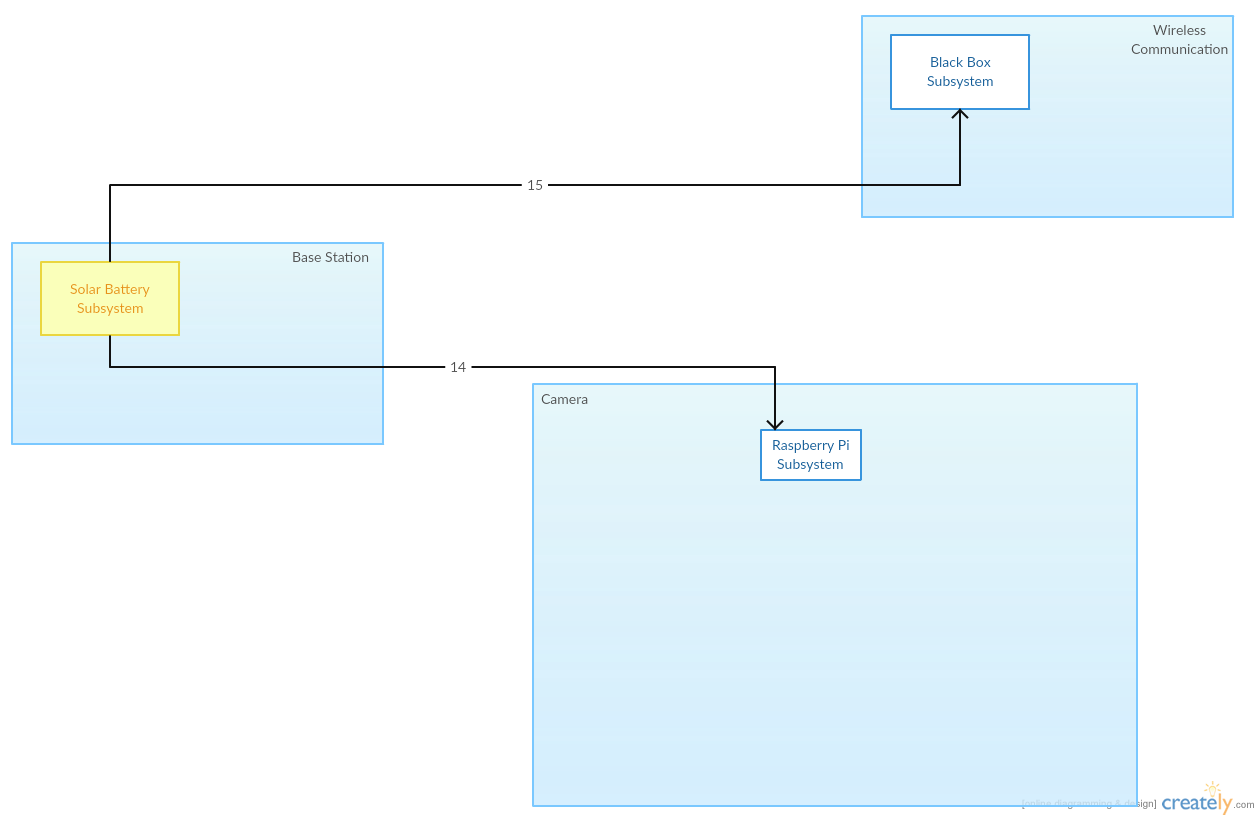
\includegraphics[width=0.60\textwidth]{images/ADSdiagrams/solarbatterysubsystem.png} 
 \caption{Camera Module Subsystem Description} 
\end{figure}

\subsubsection{Solar Battery Subsystem Hardware}
The Solar Cell is provided by TrafficNet, LLC. The Voltage Regulator is a standard incorporation of the Solar Cell which keeps the Solar Battery at a stable 5v DC which the Raspberry Pi Zero can natively utilize.

